

%% AAPT Physics Olympiad F=ma Questions
%%----------------------------------------


%% this section contains 28 problems


%% PhysicsOlympiad 2015
%%----------------------------------------


%% PhysicsOlympiad 2014
%%----------------------------------------
\element{aapt}{ %% Olympiad-A7
\begin{question}{Olympiad-2014-Q17}
    A spherical cloud of dust in space has a uniform density $\rho_0$ and a radius $R_0$.
    The gravitational acceleration of free fall at the surface
        of the cloud due to the mass of the cloud is $g_0$.
    A process occurs (heat expansion) that causes the cloud to suddenly grow to a radius $2R_0$,
        while maintaining a uniform (but not constant) density.
    The gravitational acceleration of free fall at a point $R_0$
        away from the center of the cloud due to the mass of the cloud is now:
    \begin{multicols}{3}
    \begin{choices}
        \wrongchoice{$\dfrac{1}{32} g_0$}
        \wrongchoice{$\dfrac{1}{16} g_0$}
      \correctchoice{$\dfrac{1}{8} g_0$}
        \wrongchoice{$\dfrac{1}{4} g_0$}
        \wrongchoice{$\dfrac{1}{2} g_0$}
    \end{choices}
    \end{multicols}
\end{question}
}

\element{aapt}{ %% Olympiad-A7
\begin{question}{Olympiad-2014-Q22}
    A body of mass $M$ and a body of mass $m\ll M$ are in circular orbits
        about their center of mass under the influence of their
        mutual gravitational attraction to each other.
    The distance between the bodies is $R$, which is much larger than the size of either body.
    %% Start Question
    A small amount of matter $\delta \ll m$ is removed from the body of mass $m$
        and transferred to the body of mass $M$.
    The transfer is done in such a way so that the orbits of the two bodies remain circular,
        and remain separated by a distance $R$.
    Which of the following statements is correct?
    \begin{choices}
        \wrongchoice{The gravitational force between the two bodies increases.}
        \wrongchoice{The gravitational force between the two bodies remains constant.}
        \wrongchoice{The total angular momentum of the system increases.}
        \wrongchoice{The total angular momentum of the system remains constant.}
      \correctchoice{The period of the orbit of two bodies remains constant.}
    \end{choices}
\end{question}
}


%% PhysicsOlympiad 2013
%%----------------------------------------
\element{aapt}{ %% Olympiad-A7
\begin{question}{Olympiad-2013-Q13}
    There is a ring outside of Saturn.
    In order to distinguish if the ring is actually a part of Saturn or is instead part of the satellites of Saturn,
        we need to know the relation between the velocity $v$ of each layer in the ring and the distance $R$ of the layer to the center of Saturn.
    Which of the following statements is correct?
    \begin{choices}
        %% v = \omega R, if connected
      \correctchoice{If $v\propto R$, then the layer is part of Saturn.}
        \wrongchoice{If $v^2\propto R$, then the layer is part of the satellites of Saturn.}
        \wrongchoice{If $v\propto \frac{1}{R}$, then the layer is part of Saturn.}
        %% v^2 = G M r, if in orbit
        \wrongchoice{If $v^2\propto \frac{1}{R}$, then the layer is part of Saturn.}
        \wrongchoice{If $v\propto R^2$, then the layer is part of the satellites of Saturn.}
    \end{choices}
\end{question}
}

\element{aapt}{ %% Olympiad-A7
\begin{question}{Olympiad-2013-Q16}
    %% \emph{Inspired by a problem from the 2012 International Physics Olympiad, Estonia}.
    A very large number of small particles forms a spherical cloud.
    Initially they are at rest, have uniform mass density per unit volume $\rho_0$,
        and occupy a region of radius $r_0$.
    The cloud collapses due to gravitation;
        the particles do not interact with each other in any other way.
    %% Start Questions
    How much time passes until the cloud collapses fully?
    (The constant \num{0.5427} is actually $\sqrt{\frac{3\pi}{32}}$.)
    \begin{multicols}{2}
    \begin{choices}
        %% Dimensional Analysis: time cannot depend on size
        \wrongchoice{$\dfrac{\num{0.5427}}{r_0^2 \sqrt{G\rho_0}}$}
        \wrongchoice{$\dfrac{\num{0.5427}}{r_0 \sqrt{G\rho_0}}$}
        \wrongchoice{$\dfrac{\num{0.5427}}{\sqrt{r_0 G\rho_0}}$}
      \correctchoice{$\dfrac{\num{0.5427}}{\sqrt{G\rho_0}}$}
        \wrongchoice{$\dfrac{\num{0.5427}}{\sqrt{G\rho_0}}r_0$}
    \end{choices}
    \end{multicols}
\end{question}
}

\element{aapt}{ %% Olympiad-A7
\begin{question}{Olympiad-2013-Q17}
    Two small, equal masses are attached by a lightweight rod.
    This object orbits a planet; the length of the rod is smaller than the radius of the orbit,
        but not negligible.
    The rod rotates about its axis in such a way that it remains vertical with respect to the planet.
    \begin{itemize}
        \item Is there a force in the rod?
            If so, is it tension or compression?
        \item Is the equilibrium stable, unstable, or neutral with respect to a small perturbation in the angle of the rod?
            (Assume this perturbation maintains the rate of rotation, so that in the co-rotating frame the rod is still stationary but at an angle to the vertical.)
    \end{itemize}
    \begin{center}
    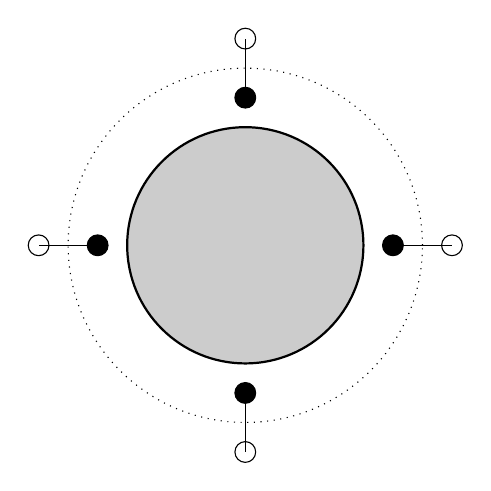
\begin{tikzpicture}[scale=0.75]
        \draw[thick,fill=white!80!black] (0,0) circle (2cm);
        \draw[dotted] (0,0) circle (3cm);
        \foreach \x in {0,90,180,270} {
            \draw[fill] (\x:2.5) circle (5pt);
            \draw (\x:3.5) circle (5pt);
            \draw (\x:2.5) -- (\x:3.5);
        }
    \end{tikzpicture}
    \end{center}
    \begin{choices}
        \wrongchoice{There is no force in the rod; the equilibrium is neutral.}
      \correctchoice{The rod is in tension; the equilibrium is stable.}
        \wrongchoice{The rod is in compression; the equilibrium is stable.}
        \wrongchoice{The rod is in tension; the equilibrium is unstable.}
        \wrongchoice{The rod is in compression; the equilibrium is unstable.}
    \end{choices}
\end{question}
}


%% PhysicsOlympiad 2012
%%----------------------------------------
\element{aapt}{ %% Olympiad-A7
\begin{question}{Olympiad-2012-Q09}
    A uniform spherical planet has radius $R$ and the acceleration due
        to gravity at its surface is $g$.
    What is the escape velocity of a particle from the planet's surface?
    \begin{multicols}{2}
    \begin{choices}
        \wrongchoice{$\frac{1}{2}\sqrt{gR}$}
        \wrongchoice{$\sqrt{gR}$}
      \correctchoice{$\sqrt{2gR}$}
        \wrongchoice{$2\sqrt{gR}$}
        \wrongchoice{The escape velocity cannot be expressed in terms of $g$ and $R$ alone.}
    \end{choices}
    \end{multicols}
\end{question}
}

\element{aapt}{ %% Olympiad-A7
\begin{question}{Olympiad-2012-Q23}
    Which of the following sets of equipment \emph{cannot} be used to
        measure the local value of the acceleration due to gravity ($g$)?
    \begin{choices}
        \wrongchoice{A spring scale (which reads in force units) and a known mass.}
        \wrongchoice{A rod of known length, an unknown mass, and a stopwatch.}
      \correctchoice{An inclined plane of known inclination, several carts of different known masses, and a stopwatch.}
        \wrongchoice{A launcher which launches projectiles at a known speed, a projectile of known mass, and a meter stick.}
        \wrongchoice{A motor with a known output power, a known mass, a piece of string of unknown length, and a stopwatch.}
    \end{choices}
\end{question}
}


%% PhysicsOlympiad 2011
%%----------------------------------------
\element{aapt}{ %% Olympiad-A7
\begin{question}{Olympiad-2011-Q12}
    You are given a large collection of identical heavy balls and lightweight rods.
    When two balls are placed at the ends of one rod and interact through
        their mutual gravitational attraction (as is shown on the left),
        the compressive force in the rod is $F$.
    \begin{center}
    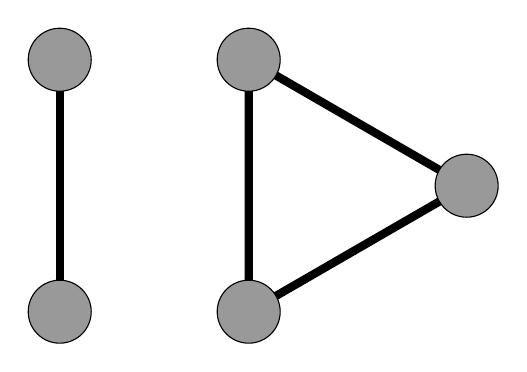
\begin{tikzpicture}[scale=0.8]
        \begin{scope}[xshift=-1.5cm]
            \draw[line width=3pt] (0,2) -- (0,1.732) -- (0,-2) --cycle;
            \draw[fill=white!60!black] (0,-2) circle (0.5cm);
            \draw[fill=white!60!black] (0,+2) circle (0.5cm);
        \end{scope}
        \begin{scope}[xshift=+1.5cm]
            \draw[line width=3pt] (0,2) -- (3.46,0) -- (0,-2) --cycle;
            \draw[fill=white!60!black] (0,-2) circle (0.5cm);
            \draw[fill=white!60!black] (0,+2) circle (0.5cm);
            \draw[fill=white!60!black] (3.46,0) circle (0.5cm);
        \end{scope}
    \end{tikzpicture}
    \end{center}
    Next,
        three balls and three rods are placed at the vertexes and edges
        of an equilateral triangle (as is shown on the right).
    What is the compressive force in each rod in the latter case?
    \begin{multicols}{3}
    \begin{choices}
        \wrongchoice{$\dfrac{1}{\sqrt{3}}F$}
        \wrongchoice{$\dfrac{\sqrt{3}}{2}F$}
      \correctchoice{$F$}
        \wrongchoice{$\sqrt{3}F$}
        \wrongchoice{$2F$}
    \end{choices}
    \end{multicols}
\end{question}
}

\element{aapt}{ %% Olympiad-A7
\begin{question}{Olympiad-2011-Q23}
    A particle is launched from the surface of a uniform,
        stationary spherical planet at an angle to the vertical.
    The particle travels in the absence of air resistance and eventually falls back onto the planet.
    Spaceman Fred describes the path of the particle as a parabola using the laws of projectile motion.
    Spacewoman Kate recalls from Kepler's laws that every bound orbit around a point mass is an ellipse (or circle),
        and that the gravitation due to a uniform sphere is identical to that of a point mass.
    Which of the following best explains the discrepancy?
    \begin{choices}
        \wrongchoice{Because the experiment takes place very close to the surface of the sphere, it is no longer valid to replace the sphere with a point mass.}
        \wrongchoice{Because the particle strikes the ground, it is not in orbit of the planet and therefore can follow a non-elliptical path.}
        \wrongchoice{Kate disregarded the fact that motions around a point mass may also be parabolas or hyperbolas.}
        \wrongchoice{Kepler's laws only hold in the limit of large orbits.}
      \correctchoice{The path is an ellipse, but is very close to a parabola due to the short length of the flight relative to the distance from the center of the planet.}
    \end{choices}
\end{question}
}


%% PhysicsOlympiad 2010
%%----------------------------------------
\element{aapt}{ %% Olympiad-A7
\begin{question}{Olympiad-2010-Q17}
    Four masses $m$ are arranged at the vertices of a tetrahedron of side length $a$.
    What is the gravitational potential energy of this arrangement?
    \begin{multicols}{2}
    \begin{choices}
        \wrongchoice{$-2\dfrac{Gm^2}{a}$}
        \wrongchoice{$-3\dfrac{Gm^2}{a}$}
        \wrongchoice{$-4\dfrac{Gm^2}{a}$}
      \correctchoice{$-6\dfrac{Gm^2}{a}$}
        \wrongchoice{$-12\dfrac{Gm^2}{a}$}
    \end{choices}
    \end{multicols}
\end{question}
}

\element{aapt}{ %% Olympiad-A7
\begin{question}{Olympiad-2010-Q21}
    The gravitational self potential energy of a solid ball
        of mass density $\rho$ and radius $R$ is $E$.
    What is the gravitational self potential energy of a ball
        of mass density $\rho$ and radius $2R$?
    \begin{multicols}{3}
    \begin{choices}
        \wrongchoice{$2E$}
        \wrongchoice{$4E$}
        \wrongchoice{$8E$}
        \wrongchoice{$16E$}
      \correctchoice{$32E$}
    \end{choices}
    \end{multicols}
\end{question}
}

\element{aapt}{ %% Olympiad-A7
\begin{question}{Olympiad-2010-Q25}
    Spaceman Fred's spaceship (which has negligible mass)
        is in an elliptical orbit about Planet Bob.
    The minimum distance between the spaceship and the planet is $R$;
        the maximum distance between the spaceship and the planet is $2R$.
    \begin{center}
    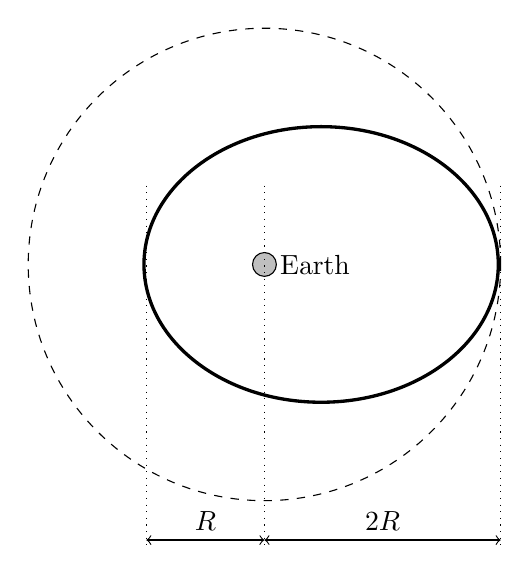
\begin{tikzpicture}
        %% Earth
        \draw[fill=white!75!black] (0,0) circle (1ex) node[anchor=west,xshift=0.5ex] {Earth};
        %% Radius
        \draw[dotted] (-1.5,1) -- (-1.5,-3.6);
        \draw[dotted] (0,1) -- (0,-3.6);
        \draw[dotted] (3,1) -- (3,-3.6);
        \draw[<->] (-1.5,-3.5) -- (0,-3.5) node[pos=0.5,anchor=south] {$R$};
        \draw[<->] (0,-3.5) -- (3,-3.5) node[pos=0.5,anchor=south] {$2R$};
        %% Inner Orbit
        \draw[very thick] (0.72,0) circle (2.25cm and 1.75cm);
        %% Outer Orbit
        \draw[dashed] (0,0) circle (3cm);
    \end{tikzpicture}
    \end{center}
    At the point of maximum distance,
        Spaceman Fred is traveling at speed $v_0$.
    He then fires his thrusters so that he enters a circular orbit of radius $2R$.
    What is his new speed?
    \begin{multicols}{2}
    \begin{choices}
      \correctchoice{$\sqrt{\dfrac{3}{2}}v_0$}
        \wrongchoice{$\sqrt{5}v_0$}
        \wrongchoice{$\sqrt{\dfrac{3}{5}}v_0$}
        \wrongchoice{$\sqrt{2}v_0$}
        \wrongchoice{$2 v_0$}
    \end{choices}
    \end{multicols}
\end{question}
}


%% PhysicsOlympiad 2009
%%----------------------------------------
\element{aapt}{ %% Olympiad-A7
\begin{question}{Olympiad-2009-Q05}
    Three equal mass satellites $A$, $B$, and $C$ are in coplanar orbits
        around a planet as shown in the figure.
    \begin{center}
    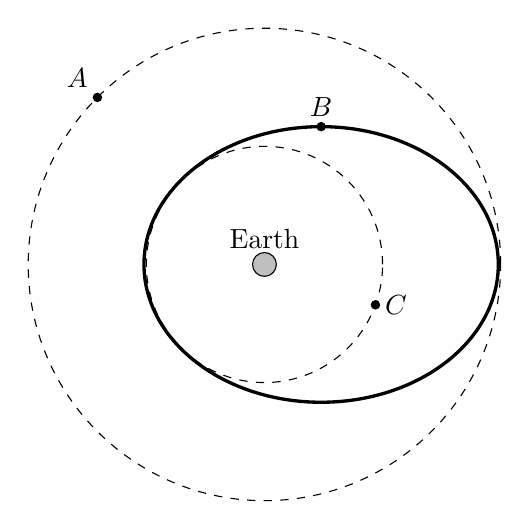
\begin{tikzpicture}
        %% Earth
        \draw[fill=white!75!black] (0,0) circle (1ex) node[anchor=south,yshift=0.5ex] {Earth};
        %% Orbit A
        \draw[dashed] (0,0) circle (3cm);
        \draw[fill] (135:3) circle (1.5pt) node[anchor=south east] {$A$};
        %% Orbit B
        \draw[very thick] (0.72,0) circle (2.25cm and 1.75cm);
        \draw[fill] (0.72,1.75) circle (1.5pt) node[anchor=south] {$B$};
        %% Orbit C
        \draw[dashed] (0,0) circle (1.5cm);
        \draw[fill] (340:1.5) circle (1.5pt) node[anchor=west] {$C$};
    \end{tikzpicture}
    \end{center}
    The magnitudes of the angular momenta of the satellites as measured
        about the planet are $L_A$, $L_B$, and $L_C$.
    Which of the following statements is correct?
    \begin{choices}
      \correctchoice{$L_A > L_B > L_C$}
        \wrongchoice{$L_C > L_B > L_A$}
        \wrongchoice{$L_B > L_C > L_A$}
        \wrongchoice{$L_B > L_A > L_C$}
        \wrongchoice{The relationship between the magnitudes is different at various instants in time.}
    \end{choices}
\end{question}
}

\newcommand{\olympiadTwentyZeroNineQTwentyOne}{
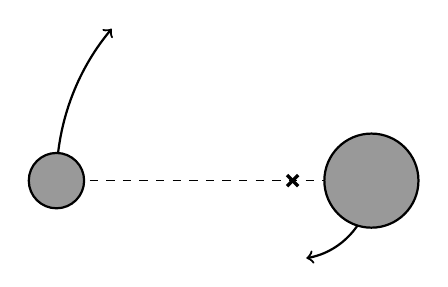
\begin{tikzpicture}
    %% Center of Mass
    \draw[very thick] (0,0) -- ++(45:0.1);
    \draw[very thick] (0,0) -- ++(135:0.1);
    \draw[very thick] (0,0) -- ++(225:0.1);
    \draw[very thick] (0,0) -- ++(315:0.1);
    %% line
    \draw[dashed] (-3,0) -- (1,0);
    %% Paths
    \draw[thick,->] (-3,0) arc(180:140:3);
    \draw[thick,->] (+1,0) arc(0:-80:1);
    %% Masses
    \draw[thick,fill=white!60!black] (-3,0) circle (10pt);
    \draw[thick,fill=white!60!black] (+1,0) circle (17pt);
\end{tikzpicture}
}

\element{aapt}{ %% Olympiad-A7
\begin{question}{Olympiad-2009-Q21}
    Two stars orbit their common center of mass as shown in the diagram below.
    The masses of the two stars are $3M$ and $M$.
    The distance between the stars is $d$.
    \begin{center}
        \olympiadTwentyZeroNineQTwentyOne
    \end{center}
    What is the value of the gravitational potential energy of the two star system?
    \begin{multicols}{2}
    \begin{choices}
        \wrongchoice{$-\dfrac{GM^2}{d}$}
        \wrongchoice{$\dfrac{3GM^2}{d}$}
        \wrongchoice{$-\dfrac{GM^2}{d^2}$}
      \correctchoice{$-\dfrac{3GM^2}{d}$}
        \wrongchoice{$-\dfrac{3GM^2}{d^2}$}
    \end{choices}
    \end{multicols}
\end{question}
}

\element{aapt}{ %% Olympiad-A7
\begin{question}{Olympiad-2009-Q22}
    Two stars orbit their common center of mass as shown in the diagram below.
    The masses of the two stars are $3M$ and $M$.
    The distance between the stars is $d$.
    \begin{center}
        \olympiadTwentyZeroNineQTwentyOne
    \end{center}
    Determine the period of the orbit for the star of mass $3M$.
    \begin{multicols}{2}
    \begin{choices}
      \correctchoice{$\pi\sqrt{\dfrac{d^3}{GM}}$}
        \wrongchoice{$\dfrac{3\pi}{4}\sqrt{\dfrac{d^3}{GM}}$}
        \wrongchoice{$\pi\sqrt{\dfrac{d^3}{3GM}}$}
        \wrongchoice{$2\pi\sqrt{\dfrac{d^3}{GM}}$}
        \wrongchoice{$\dfrac{\pi}{4}\sqrt{\dfrac{d^3}{GM}}$}
    \end{choices}
    \end{multicols}
\end{question}
}


%% PhysicsOlympiad 2008
%%----------------------------------------
\element{aapt}{ %% Olympiad-A7
\begin{question}{Olympiad-2008-Q23}
    Consider two uniform spherical planets of equal density but unequal radius.
    Which of the following quantities is the same for both planets?
    \begin{choices}
        \wrongchoice{The escape velocity from the planet's surface.}
        \wrongchoice{The acceleration due to gravity at the planet's surface.}
      \correctchoice{The orbital period of a satellite in a circular orbit just above the planet's surface.}
        \wrongchoice{The orbital period of a satellite in a circular orbit at a given distance from the planet's center.}
        \wrongchoice{None of the provided.}
    \end{choices}
\end{question}
}

\element{aapt}{ %% Olympiad-A7
\begin{question}{Olympiad-2008-Q25}
    Two satellites are launched at a distance $R$ from a planet of negligible radius.
    Both satellites are launched in the tangential direction.
    The first satellite launches correctly at a speed $v_0$ and enters a circular orbit.
    The second satellite, however, is launched at a speed $\frac{1}{2} v_0$.
    What is the minimum distance between the second satellite and the
        planet over the course of its orbit?
    \begin{multicols}{3}
    \begin{choices}
        \wrongchoice{$\dfrac{1}{\sqrt{2}}R$}
        \wrongchoice{$\dfrac{1}{2}R$}
        \wrongchoice{$\dfrac{1}{3}R$}
        \wrongchoice{$\dfrac{1}{4}R$}
      \correctchoice{$\dfrac{1}{7}R$}
    \end{choices}
    \end{multicols}
\end{question}
}


%% PhysicsOlympiad 2007
%%----------------------------------------
\element{aapt}{ %% Olympiad-A7
\begin{question}{Olympiad-2007-Q08}
    When two stars are very far apart their gravitational potential energy is zero;
        when they are separated by a distance $d$ the
        gravitational potential energy of the system is $U$.
    If the stars are separated by a distance $2d$ the
        gravitational potential energy of the system is
    \begin{multicols}{3}
    \begin{choices}
        \wrongchoice{$\frac{U}{4}$}
      \correctchoice{$\frac{U}{2}$}
        \wrongchoice{$U$}
        \wrongchoice{$2 U$}
        \wrongchoice{$4 U$}
    \end{choices}
    \end{multicols}
\end{question}
}

\element{aapt}{ %% Olympiad-A7
\begin{question}{Olympiad-2007-Q23}
    If a planet of radius $R$ spins with an angular velocity $\omega$ about an axis through the North Pole,
        what is the ratio of the normal force experienced by a person at the equator to that experienced by a person at the North Pole?
    Assume a constant gravitational field $g$ and that both people are stationary relative to the planet and are at sea level.
    \begin{multicols}{3}
    \begin{choices}
        \wrongchoice{$\dfrac{g}{R\omega^2}$}
        \wrongchoice{$\dfrac{R\omega^2}{g}$}
      \correctchoice{$1 - \dfrac{R\omega^2}{g}$}
        \wrongchoice{$1 + \dfrac{g}{R\omega^2}$}
        \wrongchoice{$1 + \dfrac{R\omega^2}{g}$}
    \end{choices}
    \end{multicols}
\end{question}
}


%% PhysicsOlympiad 2004
%%----------------------------------------


%% PhysicsOlympiad 2003
%%----------------------------------------
\element{aapt}{ %% Olympiad-A7
\begin{question}{Olympiad-2003-Q05}
    The gravitational force on a textbook at the top of Pikes Peak
        (elevation \SI{14 100}{\foot}) is \SI{40}{\newton}.
    What would be the approximate gravitational force on the same textbook if it were taken to twice the elevation?
    \begin{multicols}{3}
    \begin{choices}
        \wrongchoice{\SI{5}{\newton}}
        \wrongchoice{\SI{10}{\newton}}
        \wrongchoice{\SI{20}{\newton}}
      \correctchoice{\SI{40}{\newton}}
        \wrongchoice{\SI{80}{\newton}}
    \end{choices}
    \end{multicols}
\end{question}
}

\element{aapt}{ %% Olympiad-A7
\begin{question}{Olympiad-2003-Q12}
    A meter stick is supported at each end by a spring scale.
    A heavy mass is then hung on the meter stick so that the spring scale on the left hand side reads four times the value of the spring scale on the right hand side.
    If the mass of the meter stick is negligible compared to the hanging mass,
        how far from the right hand side is the large mass hanging?
    \begin{multicols}{3}
    \begin{choices}
        \wrongchoice{\SI{25}{\centi\meter}}
        \wrongchoice{\SI{50}{\centi\meter}}
        \wrongchoice{\SI{67}{\centi\meter}}
        \wrongchoice{\SI{75}{\centi\meter}}
      \correctchoice{\SI{80}{\centi\meter}}
    \end{choices}
    \end{multicols}
\end{question}
}


%% PhysicsOlympiad 2000
%%----------------------------------------
\element{aapt}{ %% Olympiad-A7
\begin{question}{olympiad-2000-q25}
    Two iron spheres separated by some distance have a minute gravitational attraction, $F$.
    If the spheres are moved to one half their original separation and allowed to rust so that the mass of each sphere increases \SI{41}{\percent},
        what would be the resulting gravitational force?
    \begin{multicols}{3}
    \begin{choices}
        \wrongchoice{$2F $}
        \wrongchoice{$4F $}
        \wrongchoice{$6F$}
      \correctchoice{$8F$}
        \wrongchoice{$10F$}
    \end{choices}
    \end{multicols}
\end{question}
}


%% PhysicsOlympiad 1999
%%----------------------------------------
\element{aapt}{ %% Olympiad-A7
\begin{question}{olympiad-1999-q05}
    A ball which is thrown upward near the surface of the earth with a velocity of \SI{50}{\meter\per\second} will come to rest about \SI{5}{\second} later.
    If the ball were thrown up with the same velocity on Planet $X$,
        after \SI{5}{\second} it would still be moving upwards at nearly \SI{31}{\meter\per\second}.
    The magnitude of the gravitational field near the surface of Planet $X$ is what fraction of the gravitational field near the surface of the earth?
    \begin{multicols}{3}
    \begin{choices}
        \wrongchoice{\num{0.16}}
      \correctchoice{\num{0.39}}
        \wrongchoice{\num{0.53}}
        \wrongchoice{\num{0.63}}
        \wrongchoice{\num{1.59}}
    \end{choices}
    \end{multicols}
\end{question}
}

\element{aapt}{ %% Olympiad-A7
\begin{question}{olympiad-1999-q06}
    Two light plastic shopping bags of negligible mass are placed \SI{2}{\meter} apart.
    Each bag contains 15 oranges.
    If 10 oranges were moved from one bag to the other,
        the gravitational force between the two bags would:
    \begin{choices}
        \wrongchoice{increase to $\dfrac{3}{2}$ the original value.}
        \wrongchoice{decrease to $\dfrac{2}{5}$ the original value.}
        \wrongchoice{increase to $\dfrac{5}{3}$ the original value.}
      \correctchoice{decrease to $\dfrac{5}{9}$ the original value.}
        \wrongchoice{not change.}
    \end{choices}
\end{question}
}


%% PhysicsOlympiad 1997
%%----------------------------------------
\element{aapt}{ %% Olympiad-A7
\begin{question}{olympiad-1997-q09}
    Two artificial satellites I and II have circular orbits of radii $R$ and $2R$,
        respectively, about the same planet.
    The orbital velocity of satellite I is $v$.
    What is the orbital velocity of satellite II?
    \begin{multicols}{3}
    \begin{choices}
        \wrongchoice{$\dfrac{v}{2}$}
      \correctchoice{$\dfrac{v}{\sqrt{2}}$}
        \wrongchoice{$v$}
        \wrongchoice{$\sqrt{2}v$}
        \wrongchoice{$2v$}
    \end{choices}
    \end{multicols}
\end{question}
}

\element{aapt}{ %% Olympiad-A7
\begin{question}{olympiad-1997-q10}
    The gravitational acceleration on the surface of the moon is \SI{1.6}{\meter\per\second\squared}.
    The radius of the moon is \SI{1.7e6}{\meter}.
    The period of a satellite placed in a low circular orbit about the moon is most nearly:
    \begin{multicols}{2}
    \begin{choices}
        \wrongchoice{\SI{1.0e3}{\second}}
      \correctchoice{\SI{6.5e3}{\second}}
        \wrongchoice{\SI{1.1e6}{\second}}
        \wrongchoice{\SI{5.0e6}{\second}}
        \wrongchoice{\SI{7.1e12}{\second}}
    \end{choices}
    \end{multicols}
\end{question}
}


%% PhysicsOlympiad 1994
%%----------------------------------------
\element{aapt}{ %% Olympiad-A7
\begin{question}{olympiad-1994-q08}
    An astronaut with weight $W$ on Earth lands on a planet with mass 0.1 times the mass of Earth and radius 0.5 times the radius of Earth.
    The astronaut's weight is \rule[-0.1pt]{4em}{0.1pt} on the planet.
    \begin{multicols}{3}
    \begin{choices}
        \wrongchoice{$0.02 W$}
        \wrongchoice{$0.04 W$}
        \wrongchoice{$0.2 W$}
      \correctchoice{$0.4 W$}
        \wrongchoice{$ W$}
    \end{choices}
    \end{multicols}
\end{question}
}

\element{aapt}{ %% Olympiad-A7
\begin{question}{olympiad-1994-q12}
    A rocket is launched from the surface of a planet with mass $M$ and radius $R$.
    What is the minimum velocity the rocket must be given to completely escape from the planet's gravitational field?
    \begin{multicols}{2}
    \begin{choices}
        \wrongchoice{$v = \sqrt{\dfrac{2GM}{R^2}}$}
      \correctchoice{$v = \sqrt{\dfrac{2GM}{R}}$}
        \wrongchoice{$v = \sqrt{\dfrac{GM}{R^2}}$}
        \wrongchoice{$v = \sqrt{\dfrac{GM}{R}}$}
        \wrongchoice{$v = \sqrt{GM}$}
    \end{choices}
    \end{multicols}
\end{question}
}


\endinput


